\section{Solutions to $\ls$}

The chapters of this book discussed the solution for linear systems according to various classifications. For example, does the system matrix $\A{}$ have full rank? Is the data vector $b$ in the range of the system matrix $\rng{\A{}}$? This appendix aggregates and distills all the different examples that were considered.

The lens that we are looking through here is the \svdp. It always works, but when is it the only solution? What is the role of the SVD? How is the SVD used to express solutions?

There are two classification schemes and we will relate them. The primal classification of \textit{solutions}. The number of solutions is either 0, 1 or $\infty$. The irony here is that when we encounter a linear system we typically don't know the cardinality of solutions. We usually state with the classification of \textit{systems}. Here the SVD is the universal tool which always cracks this nut open. 

%%%
\section{Classification of solutions}
First of course, the most basic fact is that every linear system will have either 0, 1 or an infinite number of solutions. More specifically these cases are characterized by these conditions.
\begin{enumerate}
\item No solution exists. The data vector is in the null space of the system matrix:
\begin{equation}
  b \in \nll{\A{}}.
\end{equation}
\item A unique point solution exists. The system matrix has full row rank
\begin{equation}
  \begin{split}
    m & = \rho,\\
    m & \le n.
  \end{split}
\end{equation}
Because the system matrix has full row rank there is no null space for the codomain and there is no place for a data vector to hide. Therefore
\begin{equation}
  b \in \rng{\A{}}.
\end{equation}
When the matrix is square $m=n$ and the standard matrix inverse exists and the solution can be cast as this:
\begin{equation}
  x=\A{-1}b.
\end{equation}
When the matrix is wide $m<n$ and the standard matrix inverse does not exist. However the pseudoinverse is a left-inverse and the point solution is written thusly:
\begin{equation}
  x=\AinvL b.
\end{equation}
\item An infinite number of solutions exist. The general solution $x_{g}$ is a particular solution (a point) $x_{p}$ and the homogeneous solution (line, plane, hyperplane, etc.) $x_{h}$:
\begin{equation}
  x_{g} = x_{p} + x_{h}
\end{equation}
The general solution is the full span of the null space of the domain. In terms of the SVD 
\begin{equation}
  x_{g} = \underbrace{\phantom{.}\mpgi{*}\, b_{\phantom{.}}}_{x_{p}=\Ap b} + \underbrace{\alpha_{1} \X{}_{\rho+1} + \dots + \alpha_{\eta_{x}} \X{}_{n}}_{x_{h}}.
\end{equation}
where the the $\alpha$ are arbitrary complex constants.
\end{enumerate}

%%%
\section{Classification of systems}
Consider the linear system where the system matrix $\Amnr$ and the data vector $b\in\cmplx{m\times 1}$. The solution vector is then $x\in\cmplx{n\times 1}$. There are three criteria used to classify solutions.
\begin{enumerate}
\item Matrix shape, $m$ rows and $n$ columns - determined by inspection:
\begin{equation*}
  \begin{array}{ll}
    m=n & \text{square} \\
    m<n & \text{tall} \\
    m>n & \text{wide}
  \end{array}
\end{equation*}
\item Matrix rank $\rho$ - the number of nonzero singular values. Usually determined reduction or computation:
\begin{equation*}
  \begin{array}{ll}
    \rho = m = n & \text{full rank} \\
    \rho = m & \text{full row rank} \\
    \rho = n & \text{full column rank}
  \end{array}
\end{equation*}
\item Data vector location - the data vector is either in the range or the null space of $\A{}$:
\begin{equation*}
  b\in\rng{\A{}} \qquad \text{ or } \qquad b\in\nll{\A{}}
\end{equation*}
\end{enumerate}
The word or here implies an exclusive or: one and only case applies.


%\section{Matrices, maps and decompositions}
Hopefully these pictures will reinforce basic concepts between matrices, their maps and their decomposition.

The three basic types of problems we considered are listed below. We will see the matrix \svdl, the transpose matrix \svdl, and the pseudoinverse expressed in terms of the decomposition matrices.
\begin{enumerate}
%
\item full rank: no rank deficits for either row or column space
\subitem no null space vectors in either $\X{}$ or $\Y{}$
\subitem both maps, $\A{}$ and $\A{T}$, are reversible
\subitem the pseudoinverse is the standard inverse
%
\item full row rank but column rank deficient
\subitem null space vectors (gray) in  $\X{}$
\subitem only the $\A{T}$ map is reversible
\subitem the pseudoinverse is a right inverse
%
\item both row and column rank deficient 
\subitem null space vectors (gray) in both $\X{}$ and $\Y{}$
\subitem neither map, $\A{}$ or $\A{T}$, is reversible
\subitem the pseudoinverse is neither a left nor a right inverse
%
\end{enumerate}



\clearpage

%%
%% 2 x 2
%%
\begin{table}[htdp]
\begin{center}
\begin{tabular}{cc}
  $\A{}x=y$ & $\A{T}y=x$\\
$\mat{rr}{1&2\\-1&2}\mat{c}{x_{1}\\x_{2}} = \mat{c}{y_{1}\\y_{2}}$ &
$\mat{rr}{1&-1\\2&2}\mat{c}{x_{1}\\x_{2}} = \mat{c}{y_{1}\\y_{2}}$ \\
\ \\
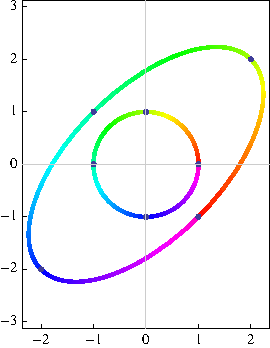
\includegraphics[ width = 2.15in ]{pdf/post_mortemII/2_2_2} &
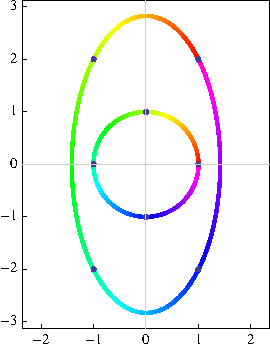
\includegraphics[ width = 2.15in ]{pdf/post_mortemII/2_2_2_t} \\
%%
\ \\
\end{tabular}
\end{center}
\label{tab:proj:a}
\caption{Case 1 - full rank: no rank deficits for either row or column space.}
\end{table}%

\begin{equation}
  \begin{array}{lcccrcr}
     \A{} &=& \svd{T} &=& \stwo \mat{rr}{1&1\\1&-1} & 
     \sqrt{2} \mat{cc}{2&0\\0&1} &
     \ktwo\\[5pt]
     \A{T} &=& \svdt{T} &=& \ktwo & \sqrt{2} \mat{cc}{2&0\\0&1} & \stwo \mat{rr}{1&1\\1&-1}\\[5pt]
     \Ap &=& \mpgi{T} &=& \ktwo & \stwo \mat{cc}{\rtwo&0\\0&1} & \stwo \mat{rr}{1&1\\1&-1}
  \end{array}
\end{equation}

\clearpage
%%
%% 2 x 3
%%
\begin{table}[htdp]
\begin{center}
\begin{tabular}{cc}
  $\A{}x=y$ & $\A{T}y=x$\\
$\mat{ccc}{0&3&0\\1&1&2}\mat{c}{x_{1}\\x_{2}\\x_{3}} = \mat{c}{y_{1}\\y_{2}}$ &
$\mat{cc}{0&1\\3&1\\0&2}\mat{c}{y_{1}\\y_{2}} = \mat{c}{x_{1}\\x_{2}\\x_{3}}$ \\
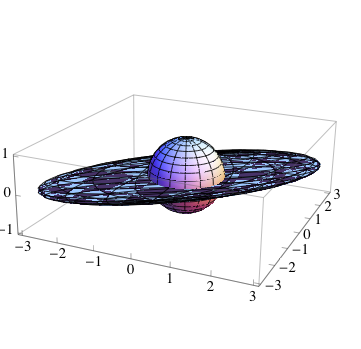
\includegraphics[ width = 2.5in ]{pdf/post_mortemII/3_2_2.png} &
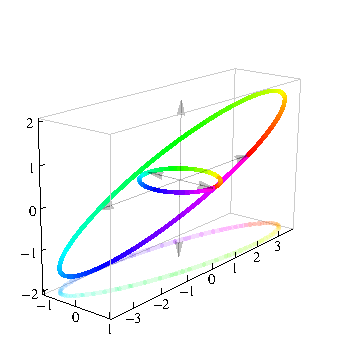
\includegraphics[ width = 2.5in ]{pdf/post_mortemII/3_2_2_t} \\
%%
\end{tabular}
\end{center}
\label{tab:proj:b}
\caption{Case 2 - full row rank but column rank deficient.}
\end{table}

%%%
\begin{equation*}
  \begin{array}{lllll}
     \svda{T} = &  \stwo
  \mat{rr}{1 & -1\\1 & 1}
  \ 
  \mat{cc|c}
  {\sqrt{15} & 0 & 0 \\
  0 & \sqrt{3}  & 0}
  \ 
  \mat{ crr }
 {\frac{1}{\sqrt{30}} & \frac{5}{\sqrt{30}} & \frac{2}{\sqrt{30}}\\
  \ssix & \frac{-1}{\sqrt{6}} & \frac{2}{\sqrt{6}} \\
  \rowcolor{ltgray}
  \frac{-2}{\sqrt{5}} & 0 & \sfive}\\
  \end{array}
\end{equation*}
%%
\begin{equation*}
  \begin{array}{lllll}
     \A{T} &= \svdt{T} = &
     \mat{rr>{\columncolor{ltgray}}r}
     { \frac{1}{\sqrt{30}} & \ssix               & \frac{-2}{\sqrt{5}} \\
       \frac{5}{\sqrt{30}} & \frac{-1}{\sqrt{6}} & 0 \\
       \frac{2}{\sqrt{30}} & \frac{2}{\sqrt{6}}  & \frac{1}{\sqrt{5}} }
     & \mat{cc}{\sqrt{15}&0\\0&\sqrt{3}\\\hline0&0} & \stwo \mat{rr}{1&1\\-1&1}\\[5pt]
  %%
     \mpgia{T} = &
     \mat{rr>{\columncolor{ltgray}}r}
     { \frac{1}{\sqrt{30}} & \ssix            & \frac{-2}{\sqrt{5}} \\
       \frac{5}{\sqrt{30}} & \frac{-1}{\sqrt{6}} & 0 \\
       \frac{2}{\sqrt{30}} & \frac{2}{\sqrt{6}}  & \frac{1}{\sqrt{5}} }
     & \mat{cc}{\frac{1}{\sqrt{15}}&0\\0&\frac{1}{\sqrt{3}}\\[5pt]\hline0&0}
     & \stwo \mat{rr}{1&1\\-1&1}
  \end{array}
\end{equation*}

\clearpage
%%
%% 3 x 2
%%
\begin{table}[htdp]
\begin{center}
\begin{tabular}{cc}
  $\A{}x=y$ & $\A{T}y=x$\\
$\Aexample \mat{c}{x_{1}\\x_{2}} = \mat{c}{y_{1}\\y_{2}\\y_{3}}$ &
$\Atexample\mat{c}{x_{1}\\x_{2}\\x_{3}} = \mat{c}{y_{1}\\y_{2}}$ \\
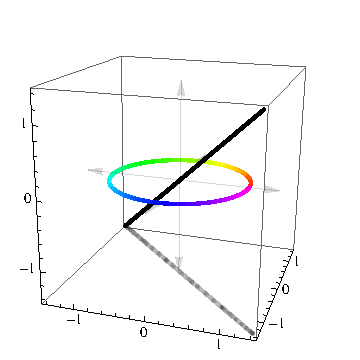
\includegraphics[ width = 2.5in ]{pdf/post_mortemII/3_2_1_a} &
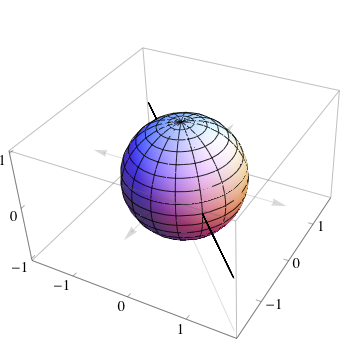
\includegraphics[ width = 2.5in ]{pdf/post_mortemII/3_2_1_t_a} \\
%%
\end{tabular}
\end{center}
\label{tab:proj:c}
\caption{Case 3 - both row and column rank deficient.}
\end{table}

\begin{equation*}
  \begin{array}{lllll}
     \A{} &= \svd{T} = &\Yshade \Sigmaexampleb \Xtshade\\
  \end{array}
\end{equation*}
\begin{equation*}
  \begin{array}{lllll}
     \A{T} &= \svdt{T} = & \Xshade & \Sigmatexamplea & \Ytshade\\[5pt]
     \mpgia{T} = & \Xshade & \Sigmainverse & \Ytshade\\
  \end{array}
\end{equation*}

\clearpage
\endinput



\endinput